Viele haben lange darauf gewartet, in Eisenach hat sich erstmals am 11. Januar  2019 eine Gruppe von 12 technisch interessierten Menschen getroffen. Sie wollen sich auch zukünftig regelmä\ss ig treffen. Es soll gemeinsam gebastelt, gelötet und programmiert werden.\\
\ \\
Zunächst haben wir uns drauf verständigt diese Treffen regelmäßig in der alten Posthalterei (Abb. \ref{img:ESAPOSTHALTEREI}) abzuhalten. Dabei werden uns die Räumlichkeiten stundenweise überlassen.\\
\ \\
\begin{minipage}[t]{\textwidth}
  \centering
  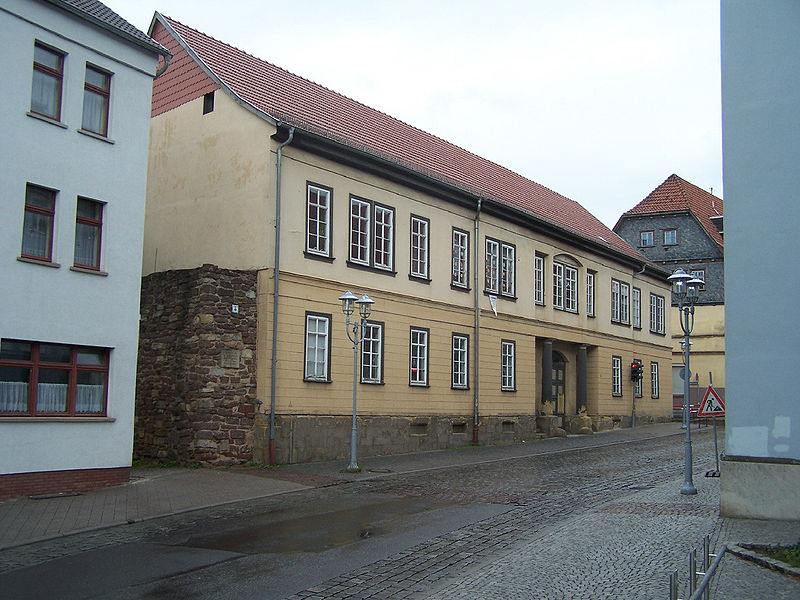
\includegraphics[height=7cm]{pictures/800px-ESAPOSTHALTEREI.jpg}
  \captionof{figure}{Alte Posthalterei}
  \label{img:ESAPOSTHALTEREI}
\end{minipage}
\ \\
Wir wollen mit einer Präsenz in sozialen Medien und mit einem Flyer (Abb. \ref{img:FlyerMitPlatine}) zunächst andere Menschen auf unsere Idee aufmerksam machen. Das weitere Vorgehen ist von der Resonanz abhängig. Ideen über Vereinsgründung und Gemeinnützigkeit bestehen, aber wir wollen bewusst dieses Thema zunächst vertagen. \\
\ \\
\begin{minipage}[t]{0.5\textwidth}
  \centering
  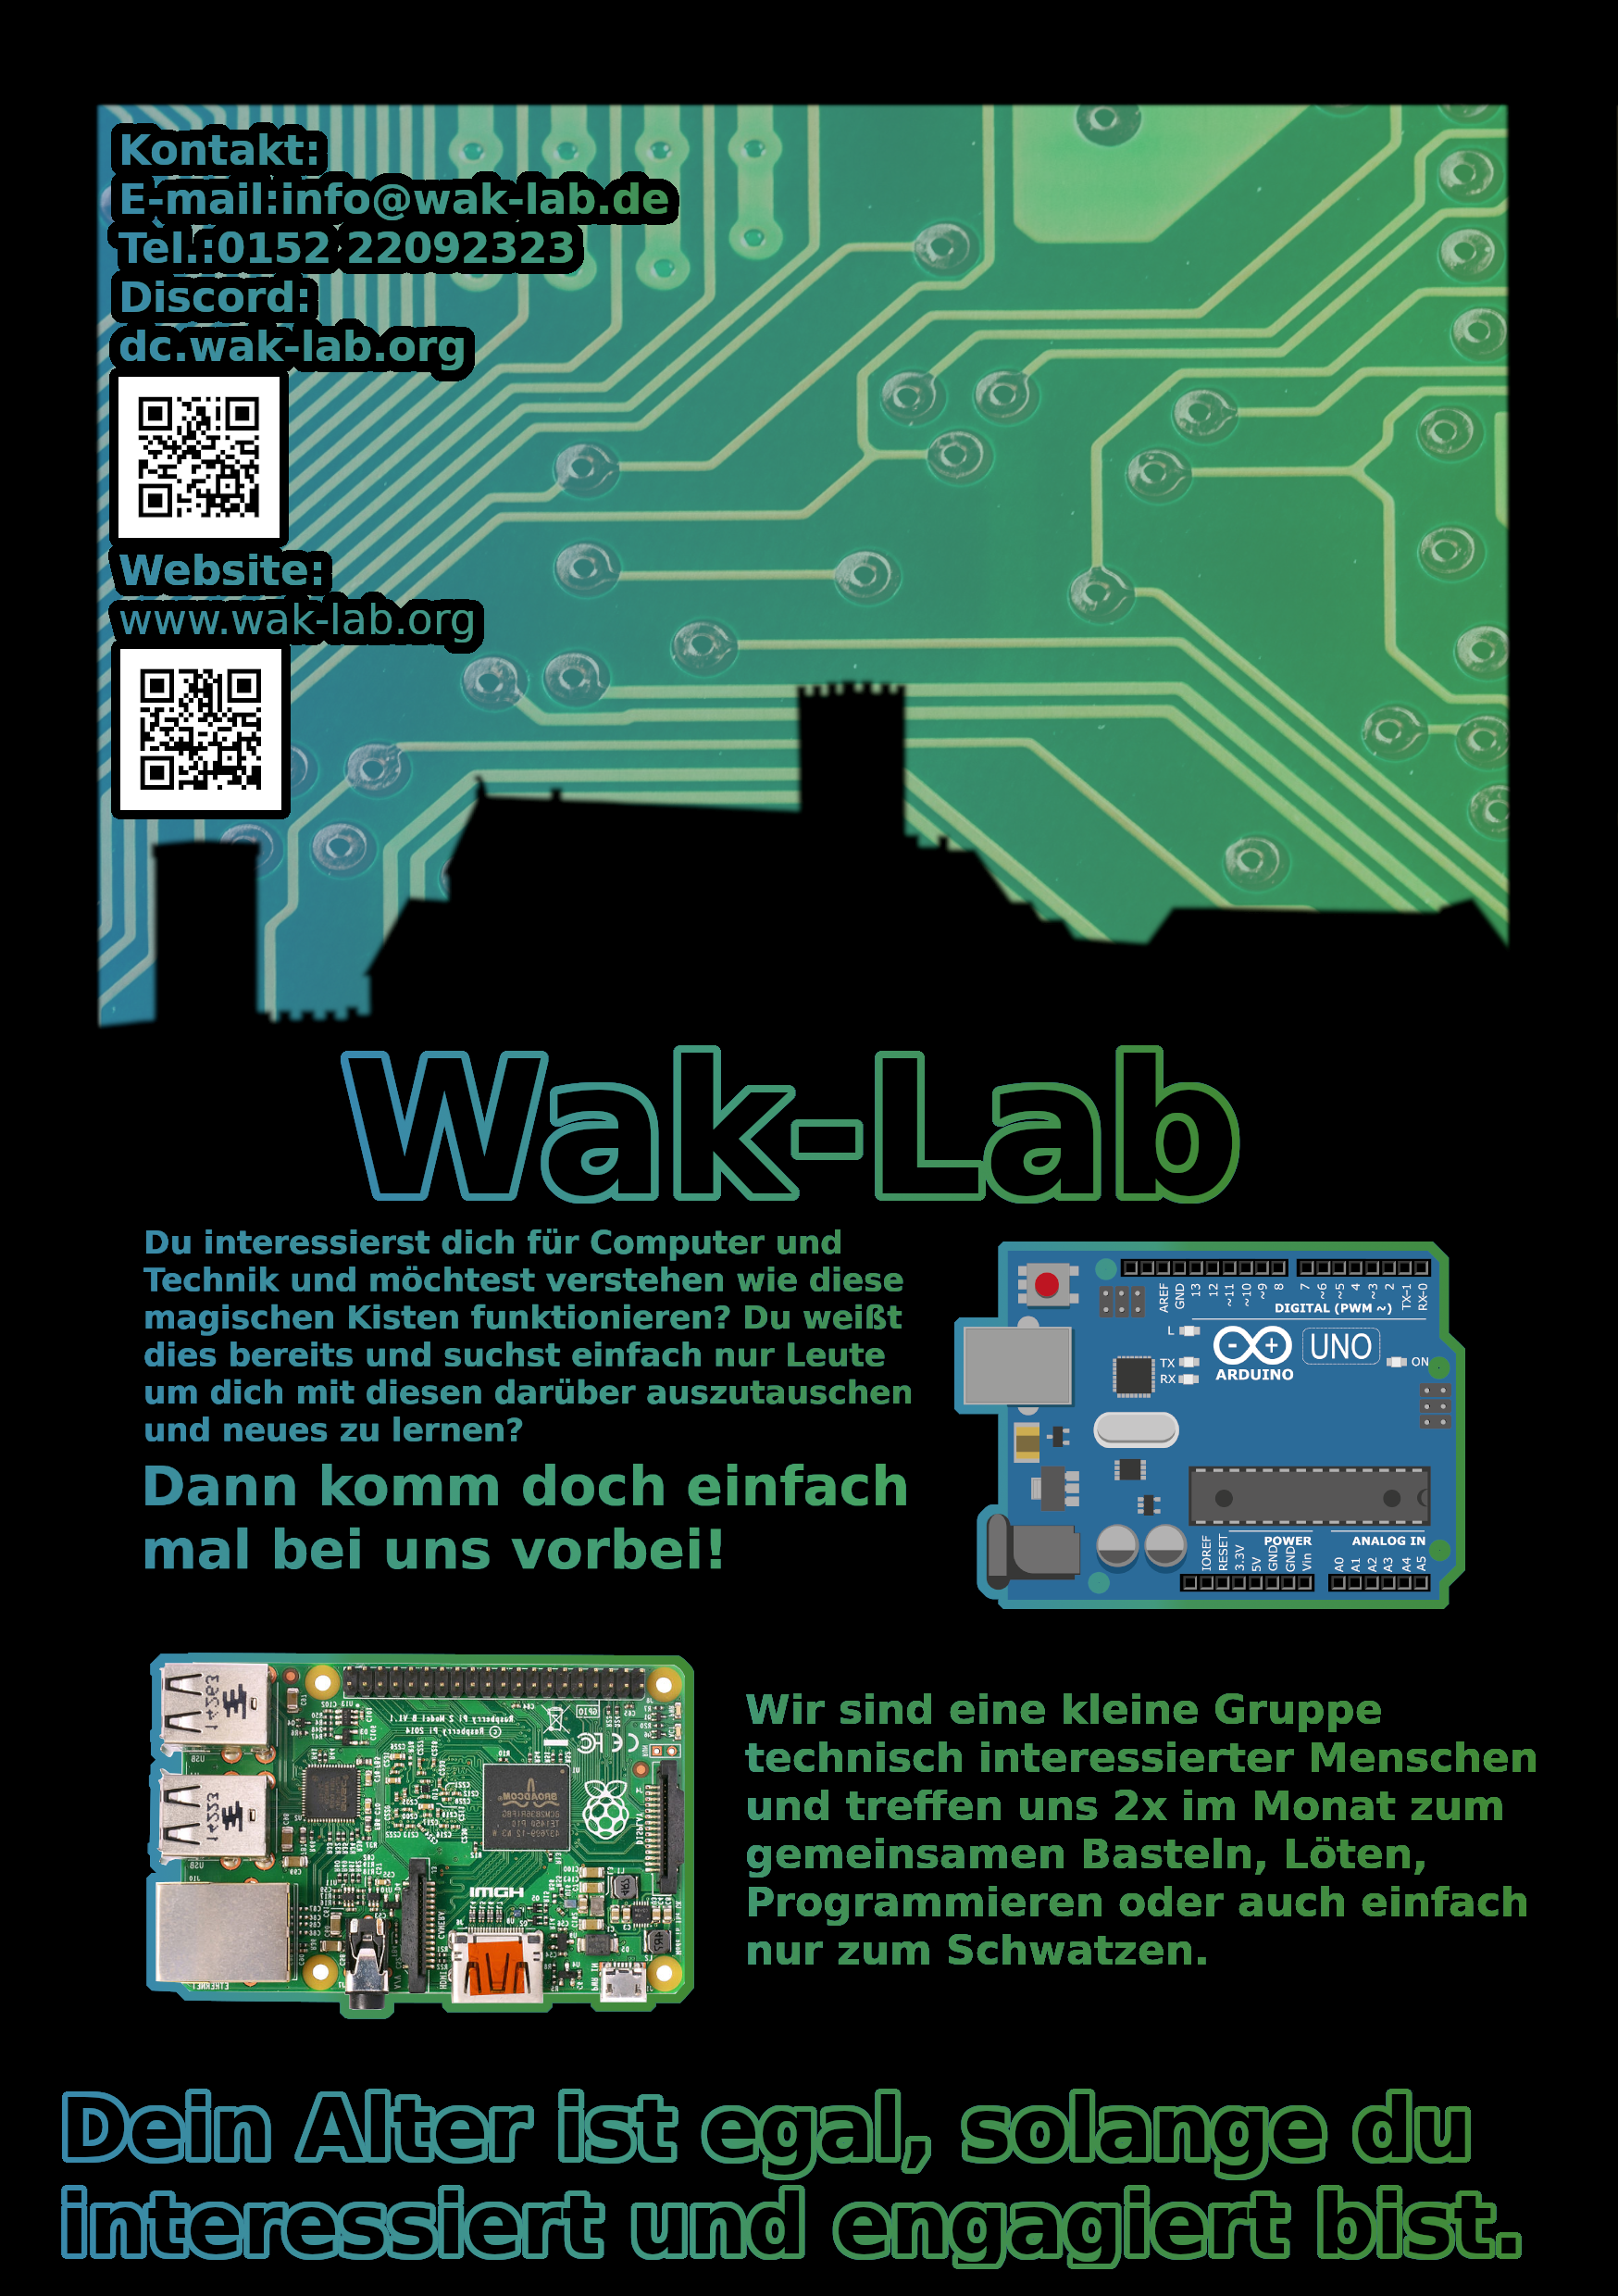
\includegraphics[height=7cm]{pictures/FlyerMitPlatine.png}
  \captionof{figure}{Flyer}
  \label{img:FlyerMitPlatine}
\end{minipage}
\begin{minipage}[t]{0.5\textwidth}
  \centering
  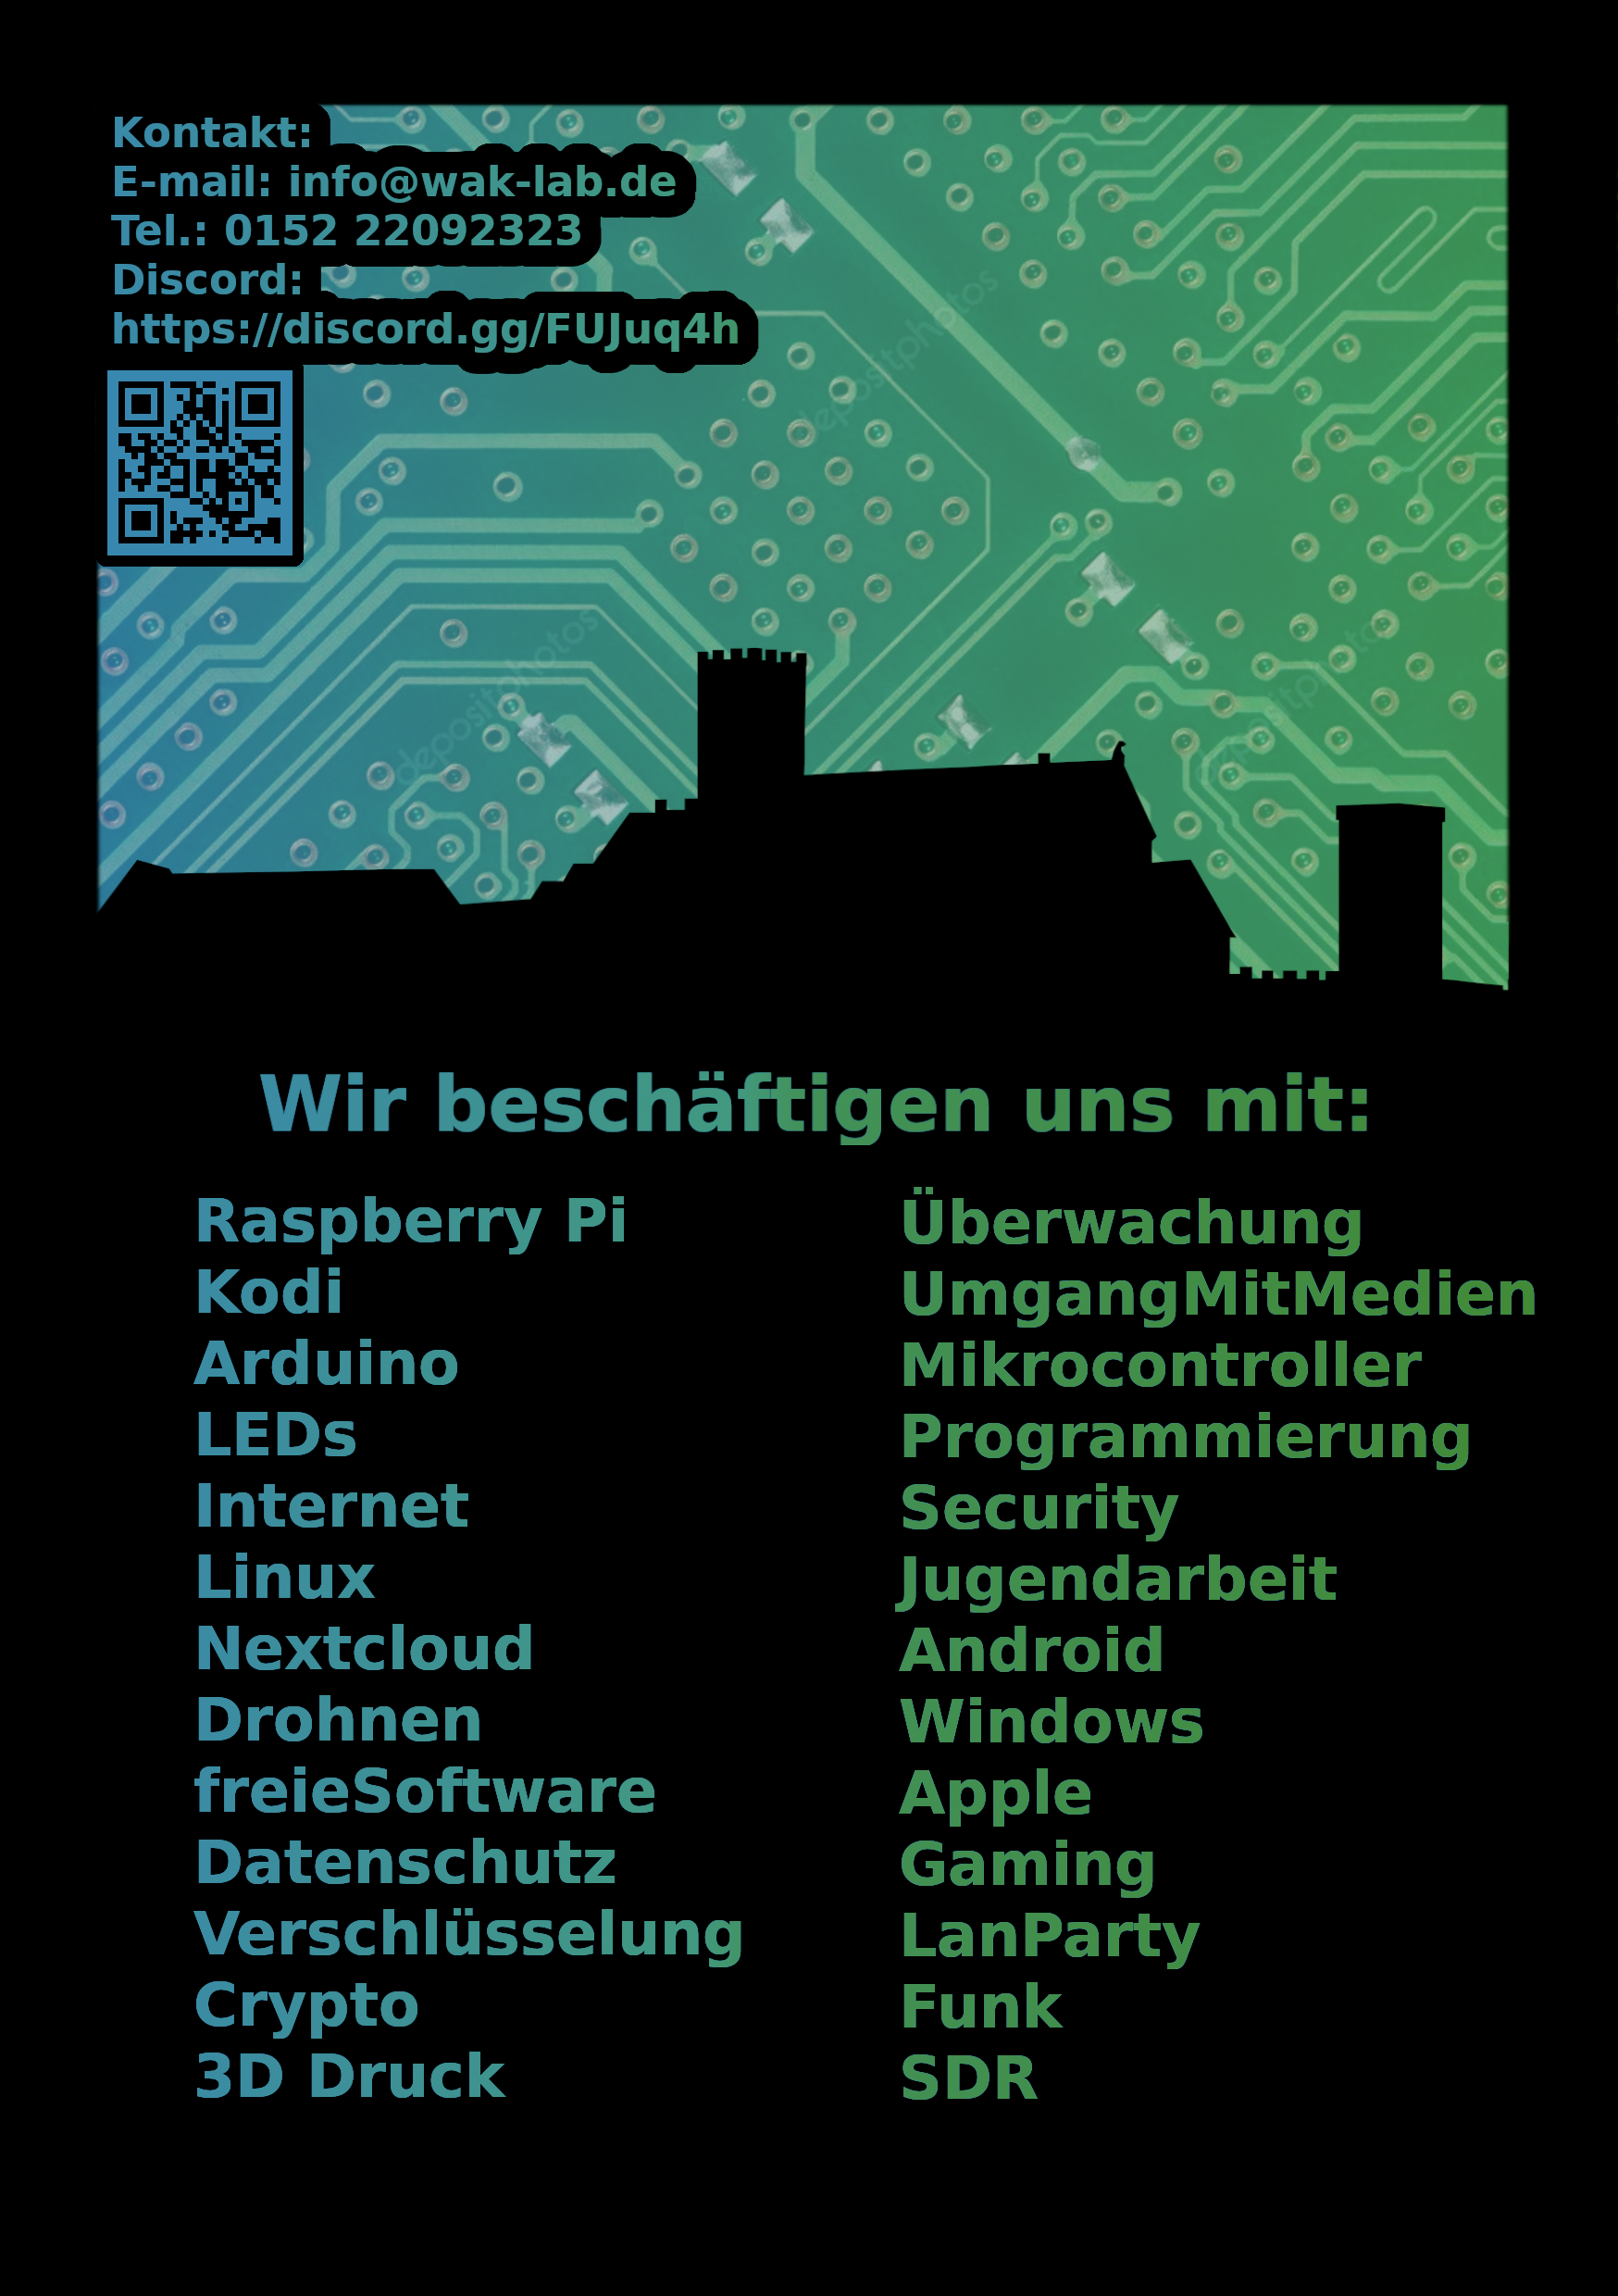
\includegraphics[height=7cm]{pictures/FlyerRueckseite.png}
  \captionof{figure}{Flyer Rückseite}
  \label{img:FlyerRueckseite}
\end{minipage}
\newpage

 
